## 最適化の方針

ここでは \ref{ss:profiling} 章で述べたように,ArchHDL::Step() と reg::Update() の処理を高速化することを考える.

最適化の方針として逐次プログラミングにおける最適化と並列化における最適化の両方を考える.


## 逐次プログラムにおける高速化手法

### データ変更の有無による条件分岐の除去 \label{sss:no_set}

\figref{src:reg} に示した実装では,reg クラスのインスタンスの値を更新する方法としてブロッキング代入とノンブロッキング代入の 2 つが存在する.

まずノンブロッキング代入について考える.reg クラスのインスタンスにノンブロッキング代入が行われた時にメンバ変数 set_ を true にし,メンバ変数 next_ に値を代入する.そして reg::Update 内では set_ が true の時だけ next_ をメンバ変数 curr_ に代入する.これは reg クラスのインスタンスの値を変更したサイクルのみで,その reg クラスのインスタンスの値を次サイクルに移る前に新しい値に更新することを意味する.

\figref{src:reg} に示した実装では,更新されない reg クラスのインスタンスの curr_ と next_ の値が同じであるため,代入する処理を行う必要はない.よって set_ 変数を用いて不要な代入を避けている.reg クラスのインスタンスの更新頻度が低い回路であればこの実装が効率的である.

次にブロッキング代入について考える.reg クラスのインスタンスにブロッキング代入が行われた時に curr_ の値を書き換える.

提案手法について述べる.この set_ 変数が true の時のみ代入するのではなく,次サイクルに移る前に next_ の値を curr_ に常に代入するようにする.こうすることによって分岐のオーバーヘッドが無くなるため,ノンブロッキング代入が頻繁に行われる回路で速度向上が期待できる.


###  \label{sss:mem_copy}

\begin{figure}[t]
 \centering
 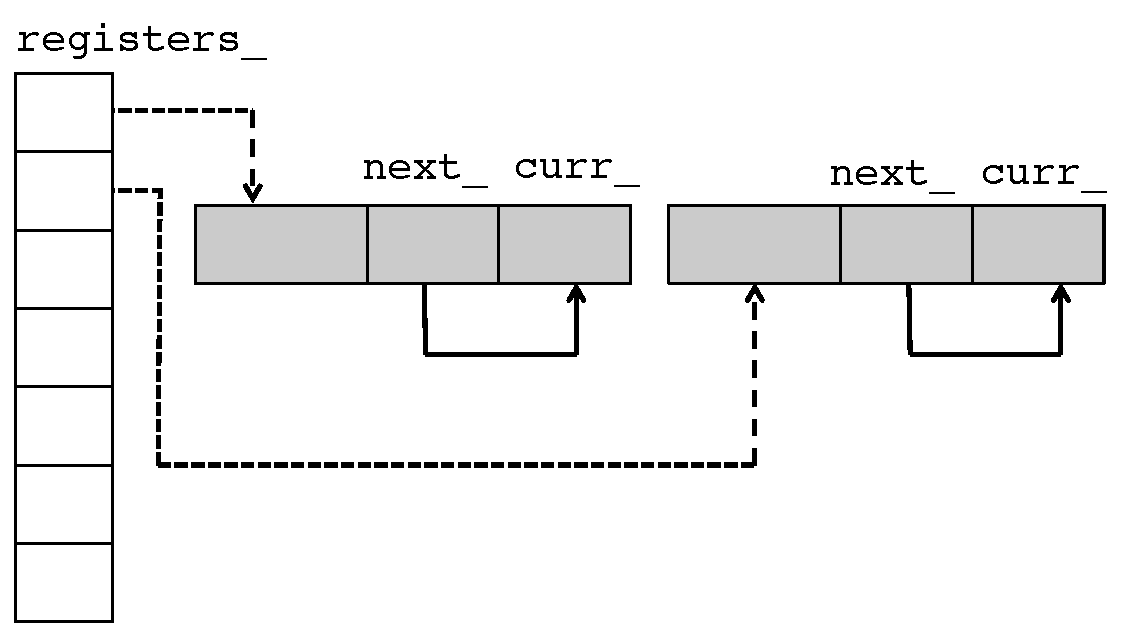
\includegraphics[clip,width=\linewidth-30pt]{simple_reg}
 \caption{シンプルな実装による reg クラスのインスタンスの処理の様子}
 \label{fig:regs}
\end{figure}

\figref{fig:regs} は現在の reg クラスのインスタンスの処理の様子である.reg インスタンスが灰色に塗られており,左からクラスのメタデータ・next_・curr_ を表している.左側の大きな枠が \figref{src:class_singleton} で示した実装の \verb`std::vector` 型の registers_ である.

\ref{sss:no_set} 節で述べたデータ変更の有無による条件分岐の除去を行うと reg::Update() メソッド内で行なっている reg クラスのインスタンスの現在の値を格納する変数に次サイクルの値を代入する処理は毎サイクル全 reg クラスのインスタンスで実行されることになる.

この代入する処理と reg::Update() メソッド自体の関数呼び出しの
2 つのオーバーヘッドが\tabref{table:stencil_prof} で示すようにArchHDL の高速化を妨げている.

\begin{figure}[t]
 \begin{center}
  \setlength{\unitlength}{1truemm} %picture環境の単位が1mmになる
\begin{picture}(70,45)(0,45)
 \put(60,82.5){\circle*{1}}
 \put(62,82.5){\circle*{1}}
 \put(64,82.5){\circle*{1}}

 \put(5,80){\framebox(20,5){}}
 \put(5,80){\color{lightgray}{\rule{20truemm}{5truemm}}}
 \put(15,80){\line(0,1){5}}
 \put(20,80){\line(0,1){5}}

 \put(13,86){\texttt{next\_}}
 \put(21,86){\texttt{curr\_}}

 \put(35,80){\framebox(20,5){}}
 \put(35,80){\color{lightgray}{\rule{20truemm}{5truemm}}}
 \put(45,80){\line(0,1){5}}
 \put(50,80){\line(0,1){5}}

 \put(15,60){\line(0,1){5}}
 \put(15,65){\line(1,0){50}}
 \put(15,60){\line(1,0){50}}
 \put(20,60){\line(0,1){5}}
 \put(25,60){\line(0,1){5}}

 \put(15,50){\line(0,1){5}}
 \put(15,55){\line(1,0){50}}
 \put(15,50){\line(1,0){50}}
 \put(20,50){\line(0,1){5}}
 \put(25,50){\line(0,1){5}}

 \put(6.5,61.5){\texttt{next\_}}
 \put(6.5,51.5){\texttt{curr\_}}

 \put(6,62){\line(-1,0){3}}
 \put(3,62){\line(0,-1){10}}
 \put(3,52){\vector(1,0){3}}


 % pointer
 \Dline(17.5,79)(17.5,67){1.1}
 \put(17.5,66){\vector(0,-1){1}}

 \Dline(23.5,79)(17.5,57){1.1}
 \put(17.5,57){\vector(-5,-22){0.5}}

 \Dline(47.5,79)(22.5,66){1.1}
 \put(22.5,66){\vector(-25,-13){1}}

 \Dline(52.5,79)(22.5,56){1.1}
 \put(22.5,56){\vector(-30,-23){1}}
\end{picture}
 \end{center}
 \caption{ reg クラスのインスタンスの処理の様子}
 \label{fig:mem_copy}
\end{figure}


そこで\figref{fig:mem_copy} のように全 reg クラスのインスタンスは現在の値と次サイクルの値の実体は持たず,ポインタを保持するようにする.実体はそれぞれ配列として持つ.\figref{fig:regs} で示すように次サイクルに移る前に行われる curr_ に next_ の値を代入する処理は registers_ から reg クラスのインスタンスが存在するアドレスを調べる必要がある.しかし \figref{fig:mem_copy} に示すようにすれば単純なメモリの並びを代入するだけになる.これにより代入する処理が高速になることが期待される.

またこの手法によって reg::Update() 自体の関数呼び出しがなくなり,関数呼び出しのオーバーヘッドがなくなる.


### ダブルバッファリング

これまでの実装では \ref{ss:implementation} 章で述べたように
reg クラスのインスタンスの次サイクルの値が次サイクルに移る前に reg クラスのインスタンスの現在の値に代入される.
そこで偶数回目の実行と奇数回目の実行で次サイクルの値と現在の値を格納している変数を
を入れ替えれば(ダブルバッファリング)代入が減ることが期待できる.

\begin{figure}[t]
 \begin{center}
  \setlength{\unitlength}{1truemm} %picture環境の単位が1mmになる
\begin{picture}(60,13)(0,-3)
 \put(10,0){\framebox(10,10){\texttt{next\_}}}
 \put(40,0){\framebox(10,10){\texttt{curr\_}}}
 \put(0,5){\vector(1,0){8}}
 \put(0,7){\texttt{write}}
 \put(22,7){\texttt{every cycle}}
 \put(22,5){\vector(1,0){16}}
 \put(22,2){\texttt{\phantom{sss}write}}
 \put(52,5){\vector(1,0){8}}
 \put(52.5,7){\texttt{read}}
\end{picture}
 \end{center}
 \caption{reg クラスのインスタンスの変数保持の処理の様子}
 \label{fig:reg_curr_next}
\end{figure}

\begin{figure}[t]
 \begin{center}
  \setlength{\unitlength}{1truemm} %picture環境の単位が1mmになる
\begin{picture}(85,33)(0,-3)
 \put(35,20){\framebox(10,10){}}
 \put(55,20){\framebox(10,10){}}
 \put(35,0){\framebox(10,10){}}
 \put(55,0){\framebox(10,10){}}
 \put(25,25){\vector(1,0){8}}
 \put(25,27){\texttt{write}}
 \put(67,25){\vector(1,0){8}}
 \put(67.5,27){\texttt{read}}
 % bottom
 \put(33,5){\vector(-1,0){8}}
 \put(25.5,7){\texttt{read}}
 \put(75,5){\vector(-1,0){8}}
 \put(67.5,7){\texttt{write}}
 % round arrow
 \qbezier(2.5,8)(0,15)(2.5,22)
 \put(2.5,22){\vector(1,2){1}}
 \put(2.5,8){\vector(1,-2){1}}
 % cycle
 \put(5,23){\texttt{odd cycle}}
 \put(5,6){\texttt{even cycle}}
\end{picture}
 \end{center}
 \caption{ダブルバッファリングの処理の様子}
 \label{fig:double_buffer}
\end{figure}

\figref{fig:reg_curr_next} はこれまでの ArchHDL の reg クラスのインスタンスの値の保持のイメージである.読み込み用と書き込み用の変数をそれぞれ保持している.読み込み用が現在の値であり,書き込み用が次サイクルの値である,次サイクルに移る前に書き込み用の値が読み込み用の変数に書き込まれる.

\figref{fig:double_buffer} はダブルバッファリングのイメージである.奇数回目のサイクルと偶数回目のサイクルで読み込み用と書き込み用の変数を入れ替える.これにより奇数回目のサイクルで書き込み用であった変数には値が書き込まれているので次サイクルの偶数回目のサイクルで読み込み用として使用出来る.これを繰り返すことで,次サイクルに移る前に行われる代入処理を無くせる.

しかし今回の手法では reg クラスのインスタンスへ値の書き込みが行われなかった場合に
reg クラスのインスタンスのその時の書き込み用の値に更新が入らない.次サイクルではその書き込み用の値がそのまま現在の値として使用されるので古い値が使われてしまう.そのため単純に入れ替えるだけの実装では誤ったシュミレーションを行なってしまう.

また今回の手法はサイクルの回数で依存関係が発生するので \ref{ss:parallel} 節で述べる並列化ができない.

よってライブラリの実装として導入するのは困難であるが,reg クラスのインスタンスへ常に書き込みが行われるカウンター回路で試したところ効果があった(具体的な数字).常に reg クラスのインスタンスに書き込みが行われるハードウェアシュミレーションを逐次処理で行いたい場合には高い効果が期待できる.

以上の理由から本論文ではダブルバッファリングによる評価は行わない.



## 並列化による高速化 \label{ss:parallel}

一方で並列化による高速化では \figref{src:class_singleton} に示すように
ArchHDL の Singleton クラスの Exec() メソッド内の
for 文内で Module::Always() メソッドと
reg::Update() メソッドは毎サイクル,各クラスの全インスタンスで呼び出されている.
モジュールの実行とレジスタの更新はそれぞれ独立に行えるので容易に並列化が可能である.

今回は for 文などの並列化を行いたい部分の前に \verb/#pragma omp/ から始まる OpenMP 指示文を与えるだけで並列化プログラミングを行える便利なライブラリである OpenMP \cite{openmp}を使用する.

\begin{figure}[t]
 \lstinputlisting[language=c++]{src/exec_openmp.cc}
 \caption{Exec メソッド内の for 文を OpenMP で並列化したプログラム}
 \label{src:exec_openmp}
\end{figure}

8 スレッドで並列化されるように OpenMP 指示文を与えたものが \figref{src:exec_openmp} である.

一般に並列化を行う場合は各スレッド対して均等に負荷を与えることが重要である.for 文の負荷を分散するスケジュール方法として静的に決定する static と,動的に決定する dynamic など複数存在する.今回の ArchHDL の場合,各モジュールと各レジスタで実行時間が大幅に変わるというのは考えにくい.よって動的に決定するオーバーヘッドを考えると static を指定した方が効率が良いと考えられる.実際に dynamic を指定すると遅くなることが確認されている.

他にも OpenMP にはオプションとしてチャンクサイズ(割り当てサイズ)を指定できる.チャンクサイズを指定するとデフォルトよりも遅くなることが確認されている(具体的な数字を載せるべき?).

よって今回の評価はスケジュール方法が static でチャンクサイズは指定しないというデフォルトの設定で行う.

